\chapter{数値実験}
\label{chap:experiment}

本章では,提案したアルゴリズムの有効性を検証するための実験を行う.
まず,提案手法とBrandes法の性能を比較する実験について説明する.
次に,第\ref{chap:complexity-analysis}章で導出した時間計算量を検証する実験の説明をする.
最後に,提案手法の応用例として,道路ネットワークを頑健にするような辺操作の探索およびその
結果について説明する.

ここで,実験で用いるネットワークについて簡単に説明する.
人工ネットワークとして,ランダム正則グラフ(以下,RRGと略記)とBarab{\'{a}}si-Albertモデル(BAと略記)を用いる.
人工ネットワークに対して,各辺に$1$から$5$までの整数をランダムに付与することで重み付きグラフとする.
実ネットワークとして,Stanford large network dataset collection\cite{Leskovec2016}から取得したネットワークを用いる.
これらのネットワークの重みを除去して,重みなしネットワークとして扱う.

すべての実験は Intel (R) Xeon (R) CPU E-2620 v4, 64GB RAM 上で行われた.
実験に用いたプログラムは gcc 7.2.0 によって, -O3 最適化フラグを付与してコンパイルされた.
プログラムのソースコードは\verb|github.com/y-satotani/dynamic-betweenness|で入手できる.

\section{Brandes法との性能比較}
はじめに,Brandes法と提案手法の性能の比較を,人工ネットワークと実ネットワークの両方の上で行う.
性能比較のため,Brandes法に対してはアルゴリズム\ref{alg:brandes}を用いて辺操作後の媒介中心性の値を計算する処理の実行時間を計測する.
また,提案手法に対してはアルゴリズム\ref{alg:proposed-algorithm-full}を用いて,
辺操作に伴う媒介中心性の値の更新に要した実行時間を計測する.

まず,人工ネットワークでの性能比較について説明する.
人工ネットワークとして,RRGとBAの両方のネットワークモデルを用いた.
ネットワークのノード数$n$は$n\in\{100,200,\ldots,1000\}$である.
各ネットワークの平均次数$k$は$k\in\{4,8\}$とした.
それぞれのネットワークの設定(ネットワークモデル,ノード数$n$,平均次数$k$の組合せ)に対して,
ネットワークを$50$個生成し,
ランダムに選択したそれぞれ$100$本の辺の挿入および削除を行った.
ここで,両アルゴリズムの終了後に操作が取り消され,ネットワークは元に戻るとする.

図\ref{fig:exp-artificial-order}はネットワークのノード数に対する
各アルゴリズムの実行時間の平均を比較したものである.
簡単のため,$k=4$の結果のみを示している.
図\ref{fig:exp-artificial-order}より,全てのネットワークモデルと辺操作に対して,
頂点数が増加するとともに提案手法の平均実行時間がBrandes法のものと比べて短くなっていることが分かる.
依存度を再計算する必要がある頂点ペアが頂点数の増加とともに比較的少なくなることが理由と考えられる.

\begin{figure}[tb]
  \centering
  \includegraphics{exp-artificial-order.pdf}
  \caption{頂点数に対する実行時間の比較}
  \label{fig:exp-artificial-order}
\end{figure}

表\ref{tab:exp-artificial}は様々な設定の人工ネットワークでの性能比較の結果を示す.
表\ref{tab:exp-artificial}より,重みなしBAネットワークなどの
いくつかのネットワークの設定において,提案手法よりBrandes法の方が実行時間が短いことがわかる.
依存度を再計算する必要がある頂点ペアが比較的少ない場合,提案手法はBrandes法に比べて,
リストのために小さなメモリ領域を割当て,解放する必要があるためと考えられる.

\input{exp-artificial.tex}

次に,実ネットワークにおける性能比較を説明する.
実ネットワークとして,Stanford large network dataset collection\cite{Leskovec2016}
から取得したネットワークを用いる.
このデータセットには,社会ネットワークや通信ネットワーク,Wikipediaのトークネットワークなど,
多種多様なネットワークが含まれている.
この中で,この実験では,コラボレーションネットワーク(次表で`ca-'から始まる)と,
%GEMSECプロジェクト\cite{Rozemberczki2019a}にて取得されたネットワーク(`gemsec-'から始まる)と,
MUSAEプロジェクト\cite{Rozemberczki2019b}にて取得されたネットワーク(`musae-'から始まる)と,
ビットコインプラットフォームでの信頼ネットワーク(`soc-sign-bitcoin'から始まる)と
%Wikipediaに関連するネットワーク(`wiki-'から始まる)を用いる.
StackExchange(`sx-'から始まる)を用いる.

各ネットワークに対して,ランダムに選択した辺の挿入および削除を$20$回繰り返した.
ここで,両アルゴリズムの終了後にネットワークは元に戻る,つまり,操作が取り消されるとする.
実ネットワークに対する性能比較の実験結果を表\ref{tab:exp-real}に示す.
表\ref{tab:exp-real}より,提案手法は実ネットワークでも効率よく計算でき,
幾何平均でおよそ$6.87$倍の性能をもつことが確認できる.

\input{exp-real.tex}

\section{導出された計算量の検証}

第\ref{chap:complexity-analysis}章で導出した計算量と,実際の実行時間と間に乖離がないか検証する.
検証のため,この実験では各アルゴリズムのステップ数を概算する.
提案手法の実行中に,影響を受ける頂点集合である$S(v)$と$T(u)$の要素数を計数した.
また,最短経路更新アルゴリズムの実行中,式\eqref{eq:average-number-of-verts-path}
で示される,影響を受ける頂点数の平均を計算する.
\begin{equation}
  \bar{A}=\frac{\sum_{s\in S(v)}|T(s)|+\sum_{t\in T(u)}|S(t)|}{|S(v)|+|T(u)|}
  \label{eq:average-number-of-verts-path}
\end{equation}
また,媒介中心性を増減させるアルゴリズムにおいて,式\eqref{eq:average-number-of-verts-betw}
で示される,アルゴリズムで走査された頂点数の平均値を計算する.
\begin{equation}
  \bar{\tau}=\frac{\sum_{s\in S(v)}|\tau(s)|+|\tau’(s)|}{2|S(v)|}
  \label{eq:average-number-of-verts-betw}
\end{equation}

これらの定義と,ネットワークの次数$k$と各アルゴリズムの計算量から,
最短経路更新アルゴリズムのステップ数を概算できる.
重みなしグラフおよび重み付きグラフにおいて,最短経路を更新するアルゴリズムのステップ数の概算は,
式\eqref{eq:full-decremental-shortest-path-update-weighted}
と式\eqref{eq:full-decremental-shortest-path-update-unweighted}から,それぞれ,
\begin{align}
  &(|S(v)|+|T(u)|)(k\bar{A}+\bar{A}\log\bar{A}),
  \label{eq:pred-path-steps-weighted} \\
  &(|S(v)|+|T(u)|)k\bar{A}.
  \label{eq:pred-path-steps-unweighted}
\end{align}
で求められる.
削除時の最短経路更新アルゴリズムについても,式\ref{eq:pred-path-steps-weighted}と
式\ref{eq:pred-path-steps-unweighted}と同一の式で算出する.

図\ref{fig:exp-artificial-path-update}は最短経路更新アルゴリズムの概算ステップ数と実行時間の
関係を示している.
概算の式の性質から,全ての頂点の次数が一定であることが望ましいため,この実験ではRRGモデルを用いた.
ネットワークのノード数は$1000$,次数は$4$とした.
この設定のネットワークを$50$個生成し,それぞれのネットワークに対して辺操作を$100$回繰り返した.
ただし,アルゴリズムの実行が完了した後,操作が取り消されネットワークが元に戻るとする.
図\ref{fig:exp-artificial-path-update}から,実行時間は概算ステップ数に線形に依存していることが
確認でき,計算量と実際の実行時間に乖離がないことが分かる.

\begin{figure}
  \centering
  \includegraphics{exp-artificial-path-update.eps}
  \caption{
    最短経路更新アルゴリズムの概算ステップ数と実行時間の関係.
    (a)は重み付きグラフでの挿入操作,(b)は重み付きグラフでの削除操作,
    (c)は重みなしグラフでの挿入操作,(d)は重みなしグラフでの削除操作の結果を示す.
    回帰直線の傾きはそれぞれ(a):$2.08\times10^{-7}$,(b):$1.59\times10^{-7}$,
    (c):$3.30\times10^{-7}$,(d):$1.26\times10^{-6}$である.
    RMSEはそれぞれ(a):$5.84\times10^{-4}$,(b):$1.85\times10^{-3}$,
    (c):$2.16\times10^{-3}$,(d):$2.81\times10^{-3}$である.
  }
  \label{fig:exp-artificial-path-update}
\end{figure}

最短経路更新アルゴリズムの時と同様に,媒介中心性を増減させるアルゴリズムに対しても
ステップ数を概算できる.
重みなしグラフおよび重み付きグラフにおいて,媒介中心性を更新するアルゴリズムのステップ数の概算は,
式\eqref{eq:full-decremental-betweenness-weighted-complexity}
と\eqref{eq:full-decremental-betweenness-unweighted-complexity}から,それぞれ,
\begin{align}
  &|S(v)|(k\bar{\tau}+\bar{\tau}\log\bar{\tau})
  \label{eq:pred-betw-steps-weighted} \\
  &|S(v)|k\bar{\tau}
  \label{eq:pred-betw-steps-unweighted}
\end{align}
で求められる.

図\ref{fig:exp-artificial-betw-update}は媒介中心性更新アルゴリズムの概算ステップ数と実行時間の
関係を示している.
最短経路更新の時と同じ理由で,この実験ではRRGモデルを用いた.
ネットワークのノード数は$1000$,次数は$4$とした.
この設定のネットワークを$50$個生成し,それぞれのネットワークに対して辺操作を$100$回繰り返した.
ただし,アルゴリズムの実行が完了した後,操作が取り消されネットワークが元に戻るとする.
図\ref{fig:exp-artificial-betw-update}から,実行時間は概算ステップ数に線形に依存していることが
確認でき,計算量と実際の実行時間に乖離がないことが分かる.

\begin{figure}
  \centering
  \includegraphics{exp-artificial-betw-update.eps}
  \caption{
    媒介中心性更新の概算ステップ数と実行時間の関係.
    (a)は重み付きグラフでの挿入操作,(b)は重み付きグラフでの削除操作,
    (c)は重みなしグラフでの挿入操作,(d)は重みなしグラフでの削除操作の結果を示す.
    回帰直線の傾きはそれぞれ(a):$4.94\times10^{-7}$,(b):$4.73\times10^{-7}$,
    (c):$4.98\times10^{-7}$,(d):$5.38\times10^{-7}$である.
    RMSEはそれぞれ(a):$2.62\times10^{-3}$,(b):$2.85\times10^{-3}$,
    (c):$1.79\times10^{-3}$,(d):$2.53\times10^{-3}$である.
  }
  \label{fig:exp-artificial-betw-update}
\end{figure}

\section{道路ネットワークを頑健にする辺操作}

%以降,本研究で提案したアルゴリズムの応用例を示す.
道路ネットワークの頑健性を向上するには
道路の建設や取り壊しによって媒介中心性の最大値を最小化し,
道路の故障に備えることが有向と考えられる.
そこで,この実験では,実際の道路ネットワークに対して一辺挿入または一辺削除を行うことによって,
媒介中心性の最大値を最小化させ,もとの道路ネットワークの頑健性を向上させる.

道路ネットワークはOpenStreetMap\cite{OpenStreetMap}を利用して独自に構築した.
実験で用いる道路ネットワークを図\ref{fig:road-okayama}に示す.
このネットワークは$12165$個の頂点と$14820$本の辺を有する.
正規化された媒介中心性の値とは,媒介中心性の値$B_x$を$(|V|-1)(|V|-2)$で割った値である.
図\ref{fig:road-okayama}の正規化された媒介中心性の最小値は$0$で,最大値は$0.1607$である.

\begin{figure}[tb]
  \centering
  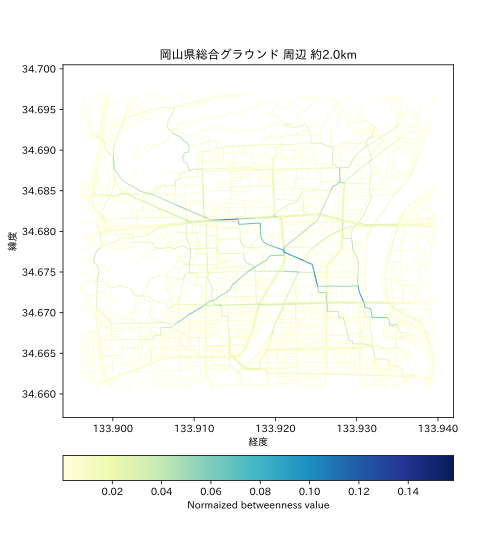
\includegraphics[width=.6\textwidth]{road-oka-with-betweenness.eps}
  \caption{
    実験で用いる道路ネットワーク
  }
  \label{fig:road-okayama}
\end{figure}

図\ref{fig:road-okayama}のネットワークのひとつの辺を操作することによって各頂点の
媒介中心性を変化させる.ネットワークから削除する辺は全ての辺$14820$本が対象で,挿入する辺は
経度と緯度の平面上において,既存のどの辺とも交わらないような辺の中から$9067$本を選択した.

図\ref{fig:exp-road-betweenness-max}はそれぞれの辺操作後の媒介中心性の
最大値の分布を表す.
最大$0.1607$の正規化された媒介中心性を
辺の挿入によって最大$0.1727$に増加,辺の削除によって最大$0.1027$に減少させることに成功した.
% 辺\{4153334442,5358091035\}を挿入,辺\{5358095473,5389817383\}を削除することによって達成される

\begin{figure}[tb]
  \centering
  \includegraphics{exp-road-betweenness-max.eps}
  \caption{辺操作時の媒介中心性の最大値の変化量.直線は操作前の媒介中心性の最大値($0.1607$)を表す.}
  \label{fig:exp-road-betweenness-max}
\end{figure}

図\ref{fig:road-oka-minimal-betweenness}と\ref{fig:road-oka-maximal-betweenness}は
それぞれ,正規化された媒介中心性を最大,最小にするような辺操作後の,
各頂点の正規化された媒介中心性の値の変化量を示す.

\begin{figure}[tb]
   \begin{minipage}{0.48\textwidth}
     \centering
     \includegraphics[width=.95\linewidth]{road-oka-minimal-betweenness.eps}
     \caption{媒介中心性の最大値を最小にする削除辺と媒介中心性の値の変化量}
     \label{fig:road-oka-minimal-betweenness}
   \end{minipage}\hfill
   \begin{minipage}{0.48\textwidth}
     \centering
     \includegraphics[width=.95\linewidth]{road-oka-maximal-betweenness.eps}
     \caption{媒介中心性の最大値を最大にする挿入辺と媒介中心性の値の変化量}
     \label{fig:road-oka-maximal-betweenness}
   \end{minipage}
\end{figure}

% \section{媒介中心性のリアルタイム計算}
% 
% 第\ref{chap:introduction}章は,社会ネットワークの分析に媒介中心性が用いられることを説明した.
% しかし,現実の社会ネットワークでは,友人関係の出現や消滅が時間とともに繰り返される.
% そのようなネットワークに対して,リアルタイムに媒介中心性を計算することは,
% 社会ネットワークの解析の観点から有用であると考えられる.
% この実験では,友人関係の出現と消滅が頻繁に発生する状況において,
% 提案手法を用いて媒介中心性をリアルタイムに計算する.
% 
% この実験では,SFHH conference data set\cite{Genois2018}というデータセットを用いた.
% このデータセットは,2009年にフランスで開催されたSFHHと呼ばれる会議の参加者に
% 赤外線タグを持たせることによって,参加者同士の交流の発生を記録したものである.
% データは20秒ごとに取得され,それぞれの時刻でどの参加者同士が近接しているかが保存されている.
% ネットワークの頂点数は$405$,辺の総数は$3509$である.
% 
% 図\ref{fig:exp-sfhh}はデータセットをもとに辺の挿入と削除を繰り返したときの,
% 提案手法とBrandes法の実行時間を表す.
% それとともに,20秒間のうちに発生した挿入辺数および削除辺数を示す.
% 図\ref{fig:exp-sfhh}より,小規模な場合ではあるが,提案手法は媒介中心性をリアルタイムに
% 計算できることが確認できる.
% しかし,更新の量が多い場合,Brandes法の方が高速に計算していることが分かる.
% 今後は,多くの辺の操作に対応するアルゴリズムの開発が求められる.
% 
% \begin{figure}[tb]
%   \centering
%   \includegraphics{exp-sfhh.eps}
%   \caption{各時刻に対する各アルゴリズムの計算時間と挿入または削除された辺数.}
%   \label{fig:exp-sfhh}
% \end{figure}
